\section{Строки: $\bs{p}$, $\bs{z}$-функции, бор, хеши}

\subsection{Префикс-функция}

\begin{definition}
    \textit{Префикс-функцией} от строки $s$ называется массив $p$, где $p_i$ равно длине самого большого префикса строки $[s_0\ldots s_i]$, который также является и её суффиксом (не считая весь $i$-й префикс).
\end{definition}

\begin{algorithm}[Кнута "---Морриса "---Пратта]
    Научимся искать подстроку $s$ в строке $t$. Пока поверим, что мы умеем считать префикс-функцию за линейное от размер строки время, и научимся с помощью неё искать подстроку в строке. Соединим подстроки $s$ и $t$ каким-нибудь символом, который не встречается ни там, ни там --- пусть это символ \texttt{\$}. Ясно, что все места, где значения перфикс-функции равны $\abs{s}$, --- это концы вхождений $s$ в текст $t$.
\end{algorithm}

Чтобы быстро считать префикс-функцию, докажем следующий факт.

\begin{lemma}
    $p_{i + 1} - p_i \leqslant 1$.
\end{lemma}

\begin{proof}
    Если есть префикс, равный суффиксу строки $[s_0\ldots s_{i + 1}]$, длины $p_{i + 1}$, то, отбросив последний символ, можно получить правильный суффикс для строки $[s_0\ldots s_i]$, длина которого будет ровно на единицу меньше.
\end{proof}

Попытаемся решить задачу с помощью динамики: найдём формулу для $p_i$ через предыдущие значения. Заметим, что $p_{i + 1} = p_i + 1$ в том и только том случае, когда $s_{p_i} = s_{i + 1}$. В этом случае мы можем просто обновить $p_{i + 1}$ и пойти дальше. Но что происходит, когда $s_{p_i} \ne s_{i + 1}$? Тогда проверяем равенство $p_{i + 1} = p_{p_i} + 1$. Если оно неверно, то проверяем $p_{i + 1} = p_{p_{p_i}} + 1$ и т.\,д. Делаем так, пока индекс не станет нулевым.

\begin{minted}[linenos, mathescape]{cpp}
vector<int> prefix_function(string s)
{
    int n = (int)s.size();
    vector<int> p(n, 0);
    for (int i = 1; i < n; ++i)
    {
        // Префикс-функция точно не больше $p_{i - 1} + 1$
        int j = p[i - 1] + 1;
        // Уменьшаем $j$, пока новый символ не подойдёт
        while (s[i] != s[j] && cur > 0)
            j = p[j - 1];
        // Здесь либо $s_i = s_{j}$, либо $j = 0$
        if (s[i] = s[j])
            p[i] = j + 1;
    }
    return p;
}
\end{minted}

В худшем случае \texttt{while} может работать за $O(n)$, но в среднем каждый \texttt{while} работает за $O(1)$.

Префикс-функция каждый шаг возрастает максимум на $1$ и после каждой итерации \texttt{while} хотя бы на $1$. Значит, суммарно операций будет не более $O(n)$.

\subsection{$z$-функция}

\begin{definition}
    \textit{$z$-функция} от строки $s$ определяется как массив $z$ такой, что $z_i$ равно длине максимальной подстроки, начинающейся с $i$-ой позиции, которая равна префиксу $s$.
\end{definition}

$z$-функцию можно использовать вместо префикс-функции в алгоритме Кнута "---Морриса "---Пратта --- только теперь нужные позиции будут начинаться с $\abs{s}$, а не заканчиваться.

Чтобы быстро считать $z$-функцию, будем идти слева направо и хранить \textit{$z$-блок} --- саму правую подстроку, равную префиксу, которую мы успели обнаружить. Будем обозначать его границы как $l$ и $r$ включительно.

Пусть мы сейчас хотим найти $z_i$, а все предыдущие уже нашли. Новый $i$-й символможет лежать либо правее $z$-блока, либо внутри него:

\begin{enumerate}[nolistsep]
    \item Если правее, то мы просто наивно перебором найдём $z_i$ (максимальный отрезок, начинающийся с $s_i$ и равный префиксу), и объявим его новым $z$-блоком;
    \item Если $i$-й элемент лежит внутри $z$-блока, то мы можем посмотреть на значение $z_{i - l}$ и использовать его, чтобы инициализировать $z_i$ чем-то, возможно, отличным от нуля. Если $z_{i - l}$ левее правой границы $z$-блока, то $z_i = z_{i - l}$ --- больше $z_i$ быть не может. Если он упирается в границу, то <<обрежем>> его до неё и будем увеличивать на $1$.
\end{enumerate}

\begin{minted}[linenos, mathescape]{cpp}
vector<int> z_function(string s)
{
    int n = (int)s.size();
    vector<int> z(n, 0);
    int l = 0, r = 0;
    for (int i = 1; i < n; ++i)
    {
        // Если мы уже видели этот символ
        if (i <= r)
        {
            // То мы можем попробовать его инициализировать
            // $z_{i - l}$, но не дальше правой границы
            z[i] = min(r - i + 1, z[i - l]);
        }
        // Дальше каждое успешное увеличение $z_i$
        // сдвинет $z$-блок на $1$
        while (i + z[i] < n && s[z[i]] == s[i + z[i]])
            ++z[i];
        if (i + z[i] - 1 > r)
        {
            r = i + z[i] - 1;
            l = i;
        }
    }
    return z;
}
\end{minted}

В алгоритме мы делаем столько же действий, сколько раз сдвигается правая граница $z$-блока, т.\,е. $O(n)$.

\subsection{Бор}

\begin{problem}
    Пусть нам дан словарь из $n$ слов $s_i$, и нам нужно отвечать на $q$ запросов вида $s$: нужно понять, если в $s$ в словаре. Можно решать бинарным поиском, тогда каждый запрос обрабатывается за $O(\abs{s}\log n)$, с помощью бора мы научимся решать задачу за $O(\abs{s})$.
\end{problem}

\subsubsection{Основная идея}

Изначально бор представляет из себя один корень. Мы хотим добавить к бору первое слово. Для этого мы добавляем его по буквам в граф (каждая буква является вершиной, рёбрами соединены вершины, если они являются соседними в каком-либо слове). А потом каждый раз, когда мы хотим добавить слово, мы идём по общему префиксу, пока можем, а затем создаём ответвление. Можно усложнять бор, например, в каждой вершине хранить количество терминальных вершин после неё (терминальная вершина --- та, в которой заканчивается слово). Тогда мы можем для любого префикса узнать количество слов с таким префиксом.

Рассмотрим пример построения бора на словаре $\{abba, abca, baba, bc, ba\}$. Будем поочерёдно добавлять слова к дереву. Изначально у нас есть только корень, к нему дописываем слово $a$ --- $b$ --- $b$ --- $a$.

\begin{center}
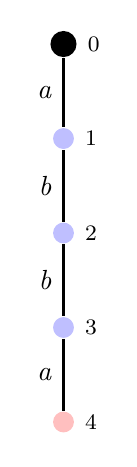
\begin{tikzpicture}[thick, level 1/.style={sibling distance=40mm}, level 2/.style={sibling distance=20mm}, level 3/.style={sibling distance=16mm}, level 4/.style={sibling distance=8mm},level 5/.style={sibling distance=4mm} xscale=-1, scale=.8]

\node[circle, fill=black] [label=right:{\footnotesize $0$}] {}
    child {node[circle,minimum width = .2cm,fill=blue!25, scale=.8] [label=right:{\footnotesize $1$}] {}
        child {node[circle,minimum width = .2cm,fill=blue!25, scale=.8] [label=right:{\footnotesize $2$}] {}
            child {node[circle,minimum width = .2cm,fill=blue!25, scale=.8] [label=right:{\footnotesize $3$}] {}
                child {node[circle,minimum width = .2cm,fill=red!25, scale=.8] [label=right:{\footnotesize $4$}] {}
                edge from parent node[left] {\textit{a}}
                }
                edge from parent node[left] {\textit{b}}
            }
            edge from parent node[left] {\textit{b}}
        }
        edge from parent node[left] {\textit{a}}
    };
\end{tikzpicture}
\end{center}

Получили такой <<бамбук>>. Теперь в дереве мы имеем перфиксы $\varnothing$ (корень), $a$, $a$ --- $b$, $a$ --- $b$ --- $b$ и $a$ --- $b$ --- $b$ --- $a$. У следующего слова с текущим деревом есть общий префикс $a$ --- $b$, поэтому мы будем не создавать новую ветку от корня, а идти по старой до конца общего префикса. Тогда наш бор приобретает следующий вид:

\begin{center}
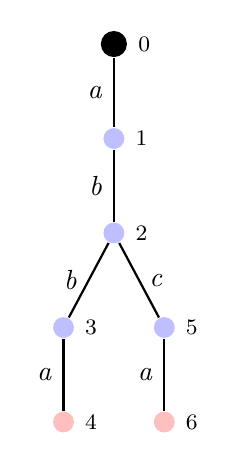
\begin{tikzpicture}[thick, level 1/.style={sibling distance=40mm}, level 2/.style={sibling distance=20mm}, level 3/.style={sibling distance=16mm}, level 4/.style={sibling distance=8mm},level 5/.style={sibling distance=4mm} xscale=-1, scale=.8]

\node[circle, fill=black] [label=right:{\footnotesize $0$}] {}
    child {node[circle,minimum width = .2cm,fill=blue!25, scale=.8] [label=right:{\footnotesize $1$}] {}
        child {node[circle,minimum width = .2cm,fill=blue!25, scale=.8] [label=right:{\footnotesize $2$}] {}
            child {node[circle,minimum width = .2cm,fill=blue!25, scale=.8] [label=right:{\footnotesize $3$}] {}
                child {node[circle,minimum width = .2cm,fill=red!25, scale=.8] [label=right:{\footnotesize $4$}] {}
            edge from parent node[left] {\textit{a}}
                }
            edge from parent node[left] {\textit{b}}
            }
            child {node[circle,minimum width = .2cm,fill=blue!25, scale=.8] [label=right:{\footnotesize $5$}] {}
                child {node[circle,minimum width = .2cm,fill=red!25, scale=.8] [label=right:{\footnotesize $6$}] {}
            edge from parent node[left] {\textit{a}}
                }
            edge from parent node[right] {\textit{c}}
            }
        edge from parent node[left] {\textit{b}}
        }
    edge from parent node[left] {\textit{a}}
    };
\end{tikzpicture}
\end{center}

Следующее слово не имеет общих префиксов с уже добавленными (на самом деле имеет, просто пустой), поэтому его подвешиваем к корню:

\begin{center}
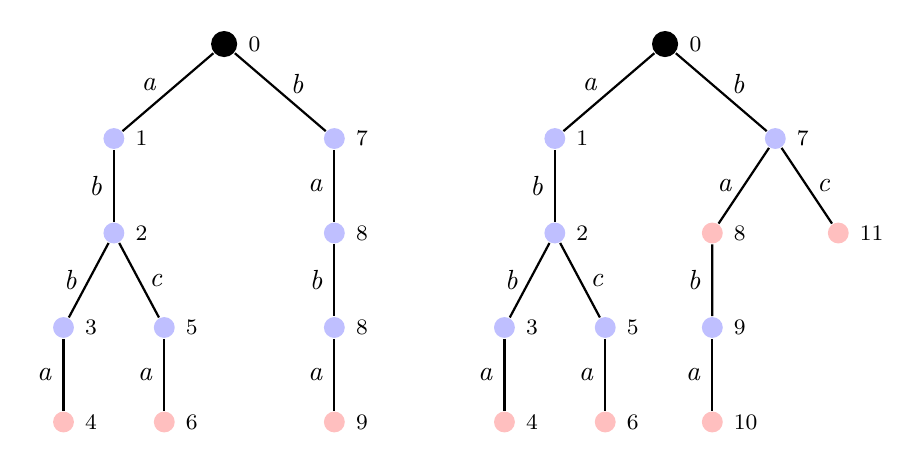
\begin{tikzpicture}[thick, level 1/.style={sibling distance=35mm}, level 2/.style={sibling distance=20mm}, level 3/.style={sibling distance=16mm}, level 4/.style={sibling distance=8mm},level 5/.style={sibling distance=4mm} xscale=-1, scale=.8]

\node[circle, fill=black] [label=right:{\footnotesize $0$}] {}
    child {node[circle,minimum width = .2cm,fill=blue!25, scale=.8] [label=right:{\footnotesize $1$}] {}
        child {node[circle,minimum width = .2cm,fill=blue!25, scale=.8] [label=right:{\footnotesize $2$}] {}
            child {node[circle,minimum width = .2cm,fill=blue!25, scale=.8] [label=right:{\footnotesize $3$}] {}
                child {node[circle,minimum width = .2cm,fill=red!25, scale=.8] [label=right:{\footnotesize $4$}] {}
            edge from parent node[left] {\textit{a}}
                }
            edge from parent node[left] {\textit{b}}
            }
            child {node[circle,minimum width = .2cm,fill=blue!25, scale=.8] [label=right:{\footnotesize $5$}] {}
                child {node[circle,minimum width = .2cm,fill=red!25, scale=.8] [label=right:{\footnotesize $6$}] {}
            edge from parent node[left] {\textit{a}}
                }
            edge from parent node[right] {\textit{c}}
            }
        edge from parent node[left] {\textit{b}}
        }
    edge from parent node[left, yshift=.1cm] {\textit{a}}
    }
    child {node[circle,minimum width = .2cm,fill=blue!25, scale=.8] [label=right:{\footnotesize $7$}] {}
        child {node[circle,minimum width = .2cm,fill=blue!25, scale=.8] [label=right:{\footnotesize $8$}] {}
            child {node[circle,minimum width = .2cm,fill=blue!25, scale=.8] [label=right:{\footnotesize $8$}] {}
                child {node[circle,minimum width = .2cm,fill=red!25, scale=.8] [label=right:{\footnotesize $9$}] {}
                edge from parent node[left] {\textit{a}}
                }
                edge from parent node[left] {\textit{b}}
            }
            edge from parent node[left] {\textit{a}}
        }
        edge from parent node[right, yshift=.1cm] {\textit{b}}
    };

\scope[xshift=7cm]
\node[circle, fill=black] [label=right:{\footnotesize $0$}] {}
    child {node[circle,minimum width = .2cm,fill=blue!25, scale=.8] [label=right:{\footnotesize $1$}] {}
        child {node[circle,minimum width = .2cm,fill=blue!25, scale=.8] [label=right:{\footnotesize $2$}] {}
            child {node[circle,minimum width = .2cm,fill=blue!25, scale=.8] [label=right:{\footnotesize $3$}] {}
                child {node[circle,minimum width = .2cm,fill=red!25, scale=.8] [label=right:{\footnotesize $4$}] {}
            edge from parent node[left] {\textit{a}}
                }
            edge from parent node[left] {\textit{b}}
            }
            child {node[circle,minimum width = .2cm,fill=blue!25, scale=.8] [label=right:{\footnotesize $5$}] {}
                child {node[circle,minimum width = .2cm,fill=red!25, scale=.8] [label=right:{\footnotesize $6$}] {}
            edge from parent node[left] {\textit{a}}
                }
            edge from parent node[right] {\textit{c}}
            }
        edge from parent node[left] {\textit{b}}
        }
    edge from parent node[left, yshift=.1cm] {\textit{a}}
    }
    child {node[circle,minimum width = .2cm,fill=blue!25, scale=.8] [label=right:{\footnotesize $7$}] {}
        child {node[circle,minimum width = .2cm,fill=red!25, scale=.8] [label=right:{\footnotesize $8$}] {}
            child {node[circle,minimum width = .2cm,fill=blue!25, scale=.8] [label=right:{\footnotesize $9$}] {}
                child {node[circle,minimum width = .2cm,fill=red!25, scale=.8] [label=right:{\footnotesize $10$}] {}
            edge from parent node[left] {\textit{a}}
                }
            edge from parent node[left] {\textit{b}}
            }
        edge from parent node[left] {\textit{a}}
        }
        child {node[circle,minimum width = .2cm,fill=red!25, scale=.8] [label=right:{\footnotesize $11$}] {}
        edge from parent node[right] {\textit{c}}
        }
    edge from parent node[right, yshift=.1cm] {\textit{b}}
    };
\endscope
\end{tikzpicture}
\end{center}

Аналогично добавляем в бор остальные слова. Заметим, что терминальные вершины (помечены красным на иллюстрациях) не обязательно должны быть листьями деревьев. Теперь научимся по данному префиксу находить количество слов с таким префиксом. Будем определять префикс по его конечной букве (конечной вершине бора). Понятно, что для листовых вершин (которые обязательно являются терминальными) ответ --- $1$. А для каждой следующей действует следующее правило: искомое число равно сумме входящих значений входящих в неё вершин. Также нужно прибавить $1$, если данная вершина является терминальной.

Следует также помнить, что бор можно строить не только на строках, а на двоичных представлениях чисел. В такой структуре вставка и поиск работают за $O(|n_2|)$, где $n_2$ --- двоичная строка, представляющая число $n$.

\subsubsection{Реализация}

\begin{minted}[linenos, mathescape]{cpp}
// нам нужны ссылки на все буквы
vector<vector<int>> link(1, vector<int>(26, -1));
// для каждой вершины отмечаем, является ли она терминальной
vector<int> marks(1, 0);

// функция для вставки слова в бор
// передаём не саму строку, а ссылку на неё, это работает за 
// $O(1)$, а не $O(|s|)$
void insert(string& s)
{
    int v = 0;
    for (int i = 0; i < int(s.size()); ++i)
    {
        int to = s[i] - 'a';
        if (link[v][to] == -1)
        {
            // Создаём новую вершину
            link.emplace_back(26, -1);
            link[v][to] = int(marks.size()) - 1;
            marks.push_back(0);
        }
        v = link[v][to]; // переходим к новой вершине
    }
    marks[v]++;
}

bool find(string& s)
{
    int v = 0;
    for (int i = 0; i < int(s.size()); ++i)
    {
        int to = s[i] - 'a';
        if (link[v][to])
            return false;
    }

    return marks[v];
}
\end{minted}

\subsection{Хеши}

\begin{definition}[\textit{Прямой полиномиальный хеш}]
    $h(s) \vcentcolon = s_0 + s_1k + s_2k^2 \hm + \ldots + s_nk^n \pmod p$, где $k$ --- произвольное число, большее размера алфавита, а $p$ --- достаточно большой модуль.
\end{definition}

Его можно подсчитать за линейное время, поддерживая переменную, равную $k$ в нужной степени:

\begin{minted}[linenos, mathescape]{cpp}
long long h = 0, m = 1;

for (char c : s)
{
    int x = (int)(c - 'a' + 1);
    h = (h + m * x) % mod;
    m = (m * k) % mod;
}
\end{minted}

Используя тот факт, что хеш --- это значение многочлена, можно быстро пересчитывать хеш от результата выполнения многих строковых операций. Например, так можно посчитать хеш от конкатенации строк $a$ и $b$: $h(ab) = h(a) + k^{\abs{a}} \cdot h(b)$. Удалить префикс строки можно так: $h(b) = \frac{h(ab) - h(a)}{k^{\abs{a}}}$, суффикс --- так: $h(a) = h(ab) - k^{\abs{a}} \cdot h(b)$.

В задачах нам часто понадобится домножать $k$ в какой-то степени, поэтому имеет смысл предпосчитать все нужные степени и сохранить в массиве $p$.

Как это использовать в реальных задачах? Пусть нам надо отвечать на запросы проверки на равенство произвольных подстрок одной большой строки. Подсчитаем значение хеш-функции для каждого префикса:

\begin{minted}[linenos, mathescape]{cpp}
vector<int> h;
h[0] = 0;

for (int i = 0; i < n; ++i)
    h[i + 1] = (h[i] + p[i] * s[i]) % mod;
\end{minted}

Теперь с помощью этих префиксных хешей мы можем определить функцию, которая будет считать хеш на любом подотрезке: $h([s_l\ldots, s_r]) \hm = \frac{h_r - h_l}{k^l}$. Деление по модулю возможно делать только при взаимно простых $k$ и модуля. В любом случае, можно этого избежать. Для нашей задачи неважно получать именно полиномиальный хеш --- достаточно, чтобы наша функция возвращала одинаковый многочлен от одинаковых подстрок. Вместо приведения к нулевой степени приведём многочлен к какой-нибудь достаточно большой, например, к $n$-й: $h([s_l\ldots s_r]) = k^{n - l}(h_r - h_l)$. Так проще --- теперь нужно домножать, а не делить:

\begin{minted}[linenos, mathescape]{cpp}
int hash_substring(int l, int r)
{
    return (h[r + 1] - h[l]) * p[n - l] % mod;
}
\end{minted}

Теперь мы можем просто вызывать эту функцию от двух отрезков и сравнивать числовое значение, отвечая на запрос за $O(1)$.

